\chapter{Variational Inference and Generative Models}
In this chapter we are going to explore some techniques that allow us to infer latent variables in latent space. We will try to understand the role of latent probabilistic models in deep learning and how to use them.

In RL, we are mostly concerned with conditional distributions $p(x|y)$ because we are trying to fit a policy function $\pi_\theta(a|s)$ which is a probabilistic model of action conditioned on state. 

So what are latent variable models? Consider that we have a very complicated distribution $p(x)$, which cannot be easily modeled by a mixture of Gaussians. By Bayes' rule, this complicated prior can be modeled by two other easier distributions:
\[
p(x) = \int p(x|z)p(z)dz
\]
$p(x|z)$ and $p(z)$ could be modeled by a conditional Gaussian and a Gaussian respectively. Since any function could be represented by a big enough neural network to an arbitrary precision, we can then use a neural net to represent $p(x|z)$ as $p(x|z) = \mathcal{N}(\mu_{nn}(z),\mu_{nn}(z))$. This sample distribution is a easy distribution with complicated parameters. Often in practice, we won't even learn $p(z)$, because we could just model it as a Gaussian distribution and transform it to any nonlinear distribution using the integral. The challenge of this approach, however, is to efficiently approximate the integral, which is quite hard.

In RL, we mainly use latent variable models in the following scenarios. First, we could use conditional latent variable models for multi-modal policies, as we discussed in imitation learning. Specifically, we could train a network with Gaussian noise to infer the state from image-based observations. Another scenario is that we could use latent variable models for model-based RL. Essentially, we learn a conditional distribution $p(o_t|x_t)$ and prior $p(x_t)$.

\section{Training Latent Variable Models}
The model we are trying to fit is $p_\theta(x)$. We train the model using data $\mathcal{D} = \{x_1,x_2,\dots,x_N\}$. We use maximum likelihood fit: $\theta\leftarrow \argmaxA_\theta\frac{1}{N}\sum_i\log p_\theta(x_i)$. Using latent variables, we have $\theta\leftarrow \argmaxA_\theta\frac{1}{N}\sum_i\log \left(\int p_\theta(x_i|z)p(z)dz \right)$. And as we have shown above, the integral is completely intractable. 

Alternatively, we could use the expected log-likelihhod:
\[
theta\leftarrow \argmaxA_\theta\frac{1}{N}\sum_i\mathbb{E}_{z\sim p(z|x_i)}\log p_\theta(x_i)
\]
However, the conditional distribution $p(z|x_i)$ is unknown. Therefore, we can approximate this distribution with a simpler distribution $q_i(z) =\mathcal{N}(\mu_i,\sigma_i)$.

\subsection{Variational Approximation}
It turns out that if we approximate the distribution using $q_i(z)$, we can bound the distribution of interest $\log p(x_i)$. Therefore, by maximizing this lower bound, we are maximizing the log likelihood. We use $q_i(z)$ to approximate $\log p(x_i)$ by:
\begin{align*}
    \log p(x_i) &= \log \int_z p(x_i|z)p(z)\\
    &= \log \int_z p(x_i|z)p(z)\frac{q_i(z)}{q_i(z)}\\
    &= \log\mathbb{E}_{z\sim q_i(z)}\left[\frac{p(x_i|z)p(z)}{q_i(z)}\right]\\
    &\geq \mathbb{E}_{z\sim q_i(z)}\left[\log \frac{p(x_i|z)p(z)}{q_i(z)}\right]\\
    &=\mathbb{E}_{z\sim q_i(z)}\left[\log p(x_i|z)+\log p(z)\right]-\mathbb{E}_{z\sim q_i(z)}\left[\log q_i(z)\right]\\
    &= \mathbb{E}_{z\sim q_i(z)}\left[\log p(x_i|z)+\log p(z)\right] + \mathcal{H}(q_i)
\end{align*}
where we applied Jensen's inequality in the second to last step. Jensen's inequality states that:
\[
\log \mathbb{E}[y] \geq \mathbb{E}[\log y]
\]

If we maximize $\log p(x_i|z)$, we will maximize $\log p(x_i)$. Also, intuitively, if we maximize $\log p(x_i|z)$, we are maximizing the peak of the distribution, and since we are maximizing the entropy $\mathcal{H}(q_i)$ too, we are also making the distribution as wide as possible, which is how we drive the approximated distribution $q_i(z)$ as close as possible to the target distribution $p(x_i,z)$.

Let us take a closer look at this lower bound. Define $\mathbb{E}_{z\sim q_i(z)}\left[\log p(x_i|z)+\log p(z)\right] + \mathcal{H}(q_i)$ as $\mathcal{L}_i(p,q_i)$. In tuitively, this term measures the likelihood. For a $q_i(z)$ to approximate $p(z|x_i)$ well, we need to minimize the KL-divergence between the two distributions. By definition, the KL divergence of the two distributions is written as:
\begin{align*}
    D_{KL}(q_i(x_i)||p(z|x_i))&=\mathbb{E}_{z\sim q_i(z)}\left[\log \frac{q_i(z)}{p(z|x_i)}\right]\\
    &=\mathbb{E}_{z\sim q_i(z)}\left[\log \frac{q_i(z)p(x_i)}{p(x_i,z)}\right]\\
    &= -\mathbb{E}_{z\sim q_i(z)}\left[\log p(x_i|z)+\log p(z)\right] + \mathbb{E}_{z\sim q_i(z)}\left[\log q_i(z)\right]+ \mathbb{E}_{z\sim q_i(z)}\left[\log p(x_i)\right]\\
    &= -\mathbb{E}_{z\sim q_i(z)}\left[\log p(x_i|z)+\log p(z)\right] -\mathcal{H}(q_i)+\log p(x_i)\\
    &=-\mathcal{L}_i(p,q_i) + \log p(x_i)
\end{align*}
Therefore,
\begin{align*}
    \log p(x_i) &= D_{KL}(q_i(z)||p(z|x_i)) + \mathcal{L}_i(p,q_i)\\
    \log p(x_i) &\geq \mathcal{L}_i(p,q_i)
\end{align*}
Note that we eliminated the expectation $\mathbb{E}_{z\sim q_i(z)}\left[\log p(x_i)\right]$ because $p(x_i)$ does not depend $z$.

Since $D_{KL}(q_i(x_i)||p(z|x_i)) = -\mathcal{L}_i(p,q_i) + \log p(x_i)$, maximizing $\mathcal{L}_i(p,q_i)$ with respect to $q_i$ minimizes the KL-divergence. Now in our maximum likelihood training, instead of doing $\theta \leftarrow \argmaxA_\theta \frac{1}{N}\sum_i \log p_\theta(x_i)$, we can use the lower bound and do $\theta \leftarrow \argmaxA_\theta \frac{1}{N}\sum_i \mathcal{L}_i(p,q_i)$ to approximate it. To optimize, for each $x_i$, we calculate $\nabla_\theta\mathcal{L}_i(p,q_i)$ by sampling $z\sim q_i(z)$ and the gradient of the likelihood term can be approximated using $\nabla_\theta\mathcal{L}_i(p,q_i)\simeq \nabla_\theta\log p_\theta(x_i|z)$ because $\log p_\theta(x_i|z)$ is the only term in the likelihood that depends on $\theta$. Then we apply gradient ascent on the parameter $\theta$ by $\theta \leftarrow \theta + \alpha\nabla_\theta\mathcal{L}_i(p,q_i)$.

However, we also need to update $q_i$ to maximize $\mathcal{L}_i(p,q_i)$ because it also depends on $\mathcal{H}(q_i)$. Let's say $q_i(z) = \mathcal{N}(\mu_i,\sigma_i)$, then we can apply gradient ascent on both parameters $\mu_i$, $\sigma_i$ to update this distribution. The problem here is the above update rule is for each data point. Therefore, the number of parameters is $|\theta| + (|\mu_i| + |\sigma_i|)*N$, where $N$ is the number of data points. Thus, we can modify the distribution we are learning so that we use a more general neural network to approximate $q(z|x_i)$ such that $q(z|x_i) = q_i(z)\simeq p(z|x_i)$. Now the number of the network parameter does not scale with the number of data points. 

\subsection{Amortized Variational Inference}
The above idea is called amortized variational inference. When we maximize the likelihood, instead of using $q_i$ for each data point, we use a general neural net $q_\phi$, parameterized by $\phi$. Then when we update $q_\phi$, we can just apply gradient ascent on $\phi$ by $\phi\leftarrow \phi + \alpha\nabla_\phi\mathcal{L}$. The likelihood can be denoted as $\mathcal{L}_i(p_\theta(x_i|z),q_\phi(z|x_i))$. 

How do we calculate $\nabla_\phi\mathcal{L}$? Note that 
\[
\mathcal{L}_i = \mathbb{E}_{z\sim q_\phi(z|x_i)}\left[\log p_\theta(x_i|z) + \log p(z)\right]+\mathcal{H}(q_\phi(z|x_i))
\]
to calculate the gradient of the likelihood with respect to $\phi$, we can calculate the entropy term's gradient easily using textbook formula. However, the first term is harder because the expectation is taken under a distribution depending on $\phi$, but the term inside the expectation is independent of $\phi$. Where have we seen this before? Where have seen the same type of gradient in policy gradient, and by applying the convenient identity, we can get the same form of gradient. If we call $\log p_\theta(x_i|z) + \log p(z)$ as $r(x_i,z)$, and $\mathbb{E}_{z\sim q_\phi(z|x_i)}$ as $J(\phi)$. Applying the same trick as in policy gradient, we can calculate $\nabla J(\phi)$ as:
\[
\nabla J(\phi)\simeq \frac{1}{M}\sum_j\nabla_\phi\log q_\phi(z_j|x_i)r(x_i,z_j)
\]
\subsection{The Reparameterization Trick}
Consider $q_\phi(z|x)$ as a Gaussian distribution $\mathcal{N}(\mu_\phi(x),\sigma_\phi(x))$, then for every $z$ in this distribution, it can be expressed as $z=\mu_\phi(x)+\epsilon\sigma_\phi(x)$, where $\epsilon$ is some type of a Gaussian noise $\epsilon \sim \mathcal{N}(0,1)$, and the noise is independent of $\phi$. Thus, we have:
\begin{align*}
    J(\phi) &= \mathbb{E}_{z\sim q_\phi(z|x_i)}[r(x_i,z)]\\
    &= \mathbb{E}_{\epsilon\sim \mathcal{N}(0,1)}\left[r(x_i,\mu_\phi(x)+\epsilon\sigma_\phi(x))\right]
\end{align*}
To estimate $\nabla_\phi J(\phi)$, we can just sample $M$ samples of $\epsilon$ from a Gaussian $\mathcal{N}(0,1)$.

Using this reparameterization trick, we can derive the expression of $\mathcal{L}_i$ in another way:
\begin{align*}
    \mathcal{L}_i &= \mathbb{E}_{z\sim q_\phi(z|x_i)}\left[\log p_\theta(x_i|z) + \log p(z)\right]+\mathcal{H}(q_\phi(z|x_i))\\
    &= \mathbb{E}_{z\sim q_\phi(z|x_i)}\left[\log p_\theta(x_i|z)\right] + \mathbb{E}_{z\sim q_\phi(z|x_i)}\left[\log p(z)\right] + \mathcal{H}(q_\phi(z|x_i))\\
    &=  \mathbb{E}_{z\sim q_\phi(z|x_i)}\left[\log p_\theta(x_i|z)\right] - D_{KL}(q_\phi(z|x_i)||p(z))\\
    &= \mathbb{E}_{\epsilon\sim \mathcal{N}(0,1)}\left[\log p_\theta(x_i|\mu_\phi(x_i)+\epsilon\sigma_\phi(x_i))\right] - D_{KL}(q_\phi(z|x_i)||p(z))\\
    &\simeq \log p_\theta( x_i|\mu_\phi(x_i)+\epsilon\sigma_\phi(x_i)) - D_{KL}(q_\phi(z|x_i)||p(z))
\end{align*}
The complete computational graph for variational inference is shown in Fig. \ref{fig:varinf}. 
\begin{figure}
    \centering
    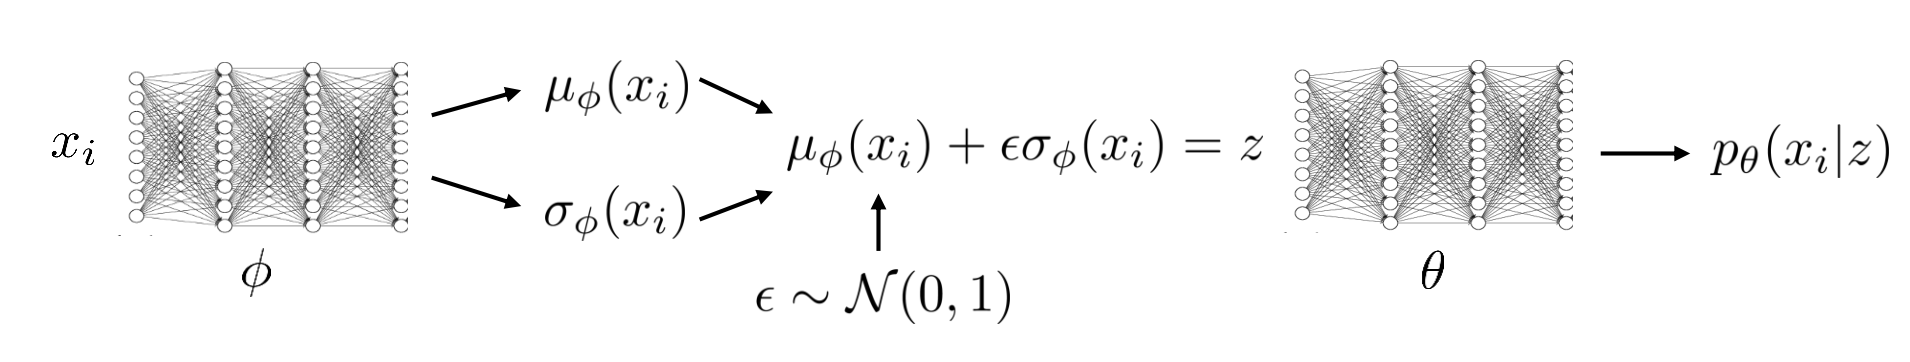
\includegraphics[scale=0.4]{figures/varinf.png}
    \caption{Variational inference}
    \label{fig:varinf}
\end{figure}

Compared with policy gradient, the reparameterization trick is easy to implement and as low variance, but it only works for continuous latent variables. Policy gradient can Can handle both discrete and continuous latent variables, but it is subject to high variance, rand equires multiple samples and small learning rates.

\section{Variational Autoencoder (VAE)}
The variational autoencoder (VAE) consists of two parts: an encoder and a decoder. The encoder $q_\phi(z|x) = \mathcal{N}(\mu_\phi(x),\sigma_\phi(x))$ parameterized by $\phi$ gives us a latent variable $z$, and the decoder $p_\theta(x|z) = \mathcal{N}(\mu_\theta(x),\sigma_\theta(x))$ is parameterized by $\theta$.

When we are inferring $p(x)$ by $p(x) = \int p(x|z)p(z)dz$, we sample $z$ from the distribution $p(z)$, and sample $x$ from the distribution $p(x|z)$. Why does this work? Recall the evidence lower bound $\mathcal{L}_i$ is defined as:
\[
\mathcal{L}_i=  \mathbb{E}_{z\sim q_\phi(z|x_i)}\left[\log p_\theta(x_i|z)\right] - D_{KL}(q_\phi(z|x_i)||p(z))
\]
$q_\phi$ should embed your observations $x_i$ into $z$, into a distribution that is closer to the prior. So if the training data is embedded into the distribution that is similar to the prior, it makes sense that the samples from the prior will give you things that look like the data.
\begin{figure}[H]
    \centering
    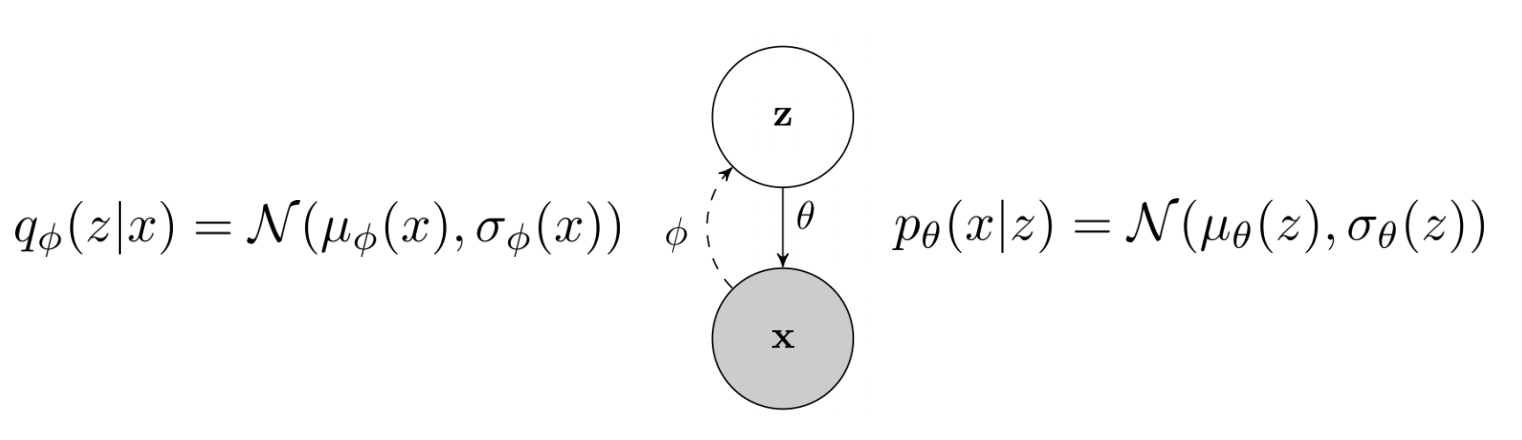
\includegraphics[scale=0.4]{figures/vae.png}
    \caption{VAE}
    \label{fig:vae}
\end{figure}